\section{Introduction}

    \subparagraph{}Le but de ce {\color{info}premier travail} est d'implémenter un circuit contenant au moins une source de tension ainsi qu'une source de courant avec 
    plusieurs résistances. Il s'agira ensuite de calculer les tensions, courants et puissances du circuit et enfin de simuler le circuit avec le logiciel \textit{LTspice}
    afin de démontrer l'exactitude des calculs.\\[1.5cm]
    
    \begin{titletbox}{À l'attention du correcteur / correctrice}{warning}
        N'hésitez pas à zoomer sur les schémas du circuit et autres images afin d'y voir plus clair.
    \end{titletbox}

\section{Schéma initial du circuit}

    \begin{figure}[H]
        \centering
        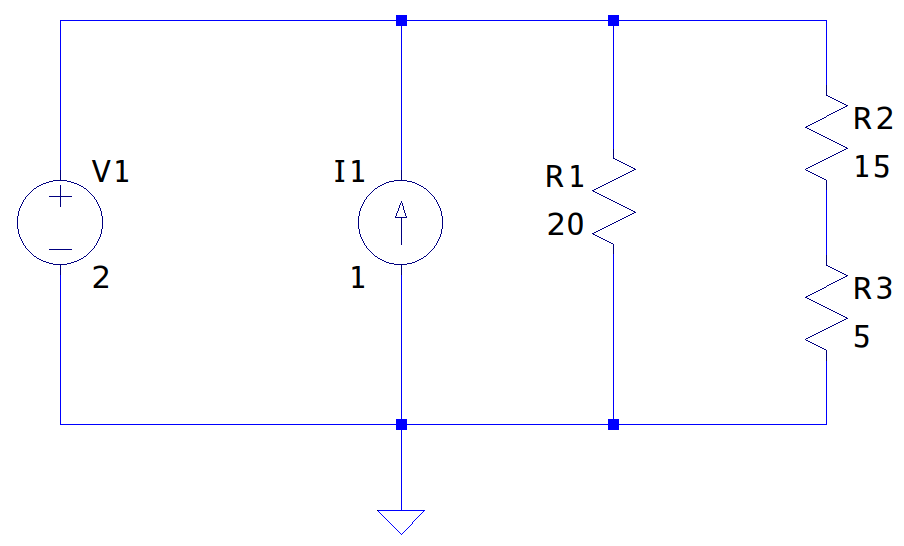
\includegraphics[scale=0.7]{../pictures/circuit.png} % Pas utiliser width=\textwidth pcq il prend la taille de \section{} comme ref
        \caption{Schéma du circuit}
    \end{figure}

    \begin{figure}[H]
        \centering
        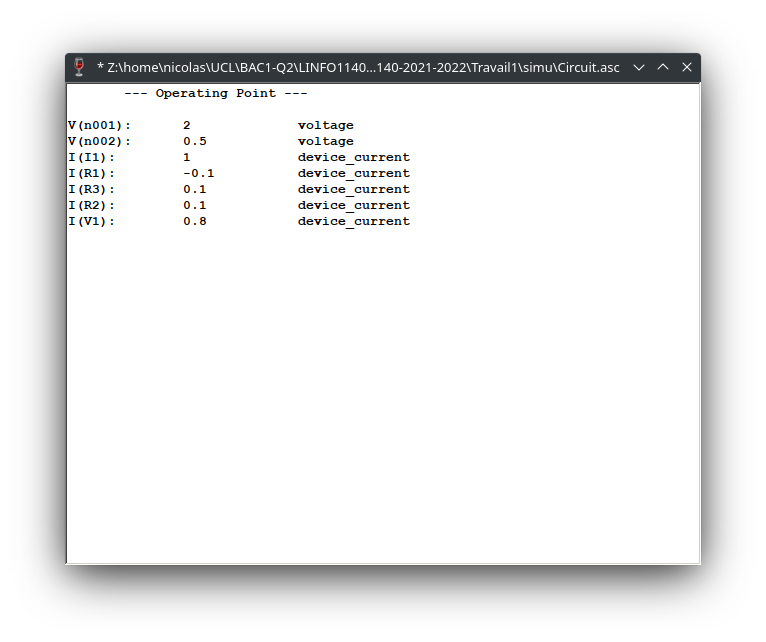
\includegraphics[scale=0.5]{../pictures/resultat.png} % Pas utiliser width=\textwidth pcq il prend la taille de \section{} comme ref
        \caption{Résultat du circuit}
    \end{figure}




\section{Calculs}

\subsection{Simplification du circuit initial}

    \paragraph{}Je vais commencer par simplifier toutes les résistances présente dans le circuit. On aperçoit que
    $R_2$ et $R_3$ sont en série et que $R_1$ est en parallèle avec ces deux dernières. La résistance équivalente vaut 
    donc : 

        {\color{info}\begin{align*}
            R_{eq}\;&=\;R_{1}\;//\;(R_{2}\;+\;R_{3}) \\
            R_{eq}\;&=\;20\;//\;(15\;+\;5) \\
            R_{eq}\;&=\;20\;//\;20
        \end{align*}}
        

        \begin{empheq}[box=\fbox]{equation*}
            \color{red}
            R_{eq}\;=10\;\Omega
        \end{empheq}

    \paragraph{}Nous obtenons donc le circuit suivant :

    \begin{figure}[H]
        \centering
        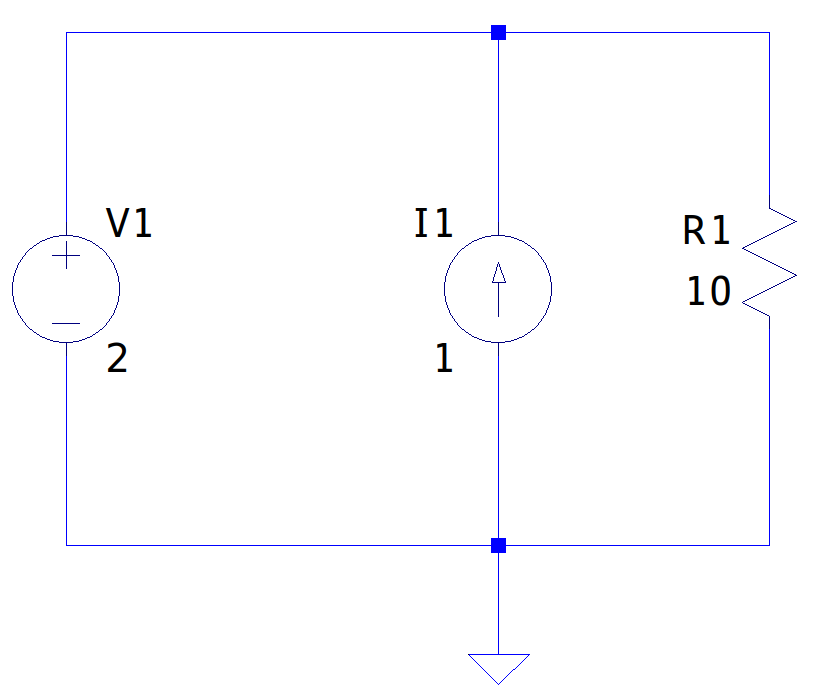
\includegraphics[width=0.7\textwidth]{../pictures/simple.png} % Pas utiliser width=\textwidth pcq il prend la taille de \section{} comme ref
        \caption{Circuit simplifié}
    \end{figure}

    \paragraph{}Grâce à la loi des noeuds, nous savons déjà qu'il y a une différence de potentiel de 2V aux bornes de la
    résistance équivalente ($R_{eq}$). Le courant passant par $R_eq$ vaut donc :

        {\color{info}\begin{align*}
            I_{R_{eq}}\;&=\frac{V}{R} \\
            I_{R_{eq}}\;&=\frac{2}{10} \\
            I_{R_{eq}}\;&=0.2
        \end{align*}}
        

        \begin{empheq}[box=\fbox]{equation*}
            \color{red}
            I_{R_{eq}}\;=200\;mA
        \end{empheq}


\subsection{Recomposition du circuit}

    \paragraph{}Je vais maintenant recomposer le circuit, annoté avec les informations que nous connaissons :


    \begin{figure}[H]
        \centering
        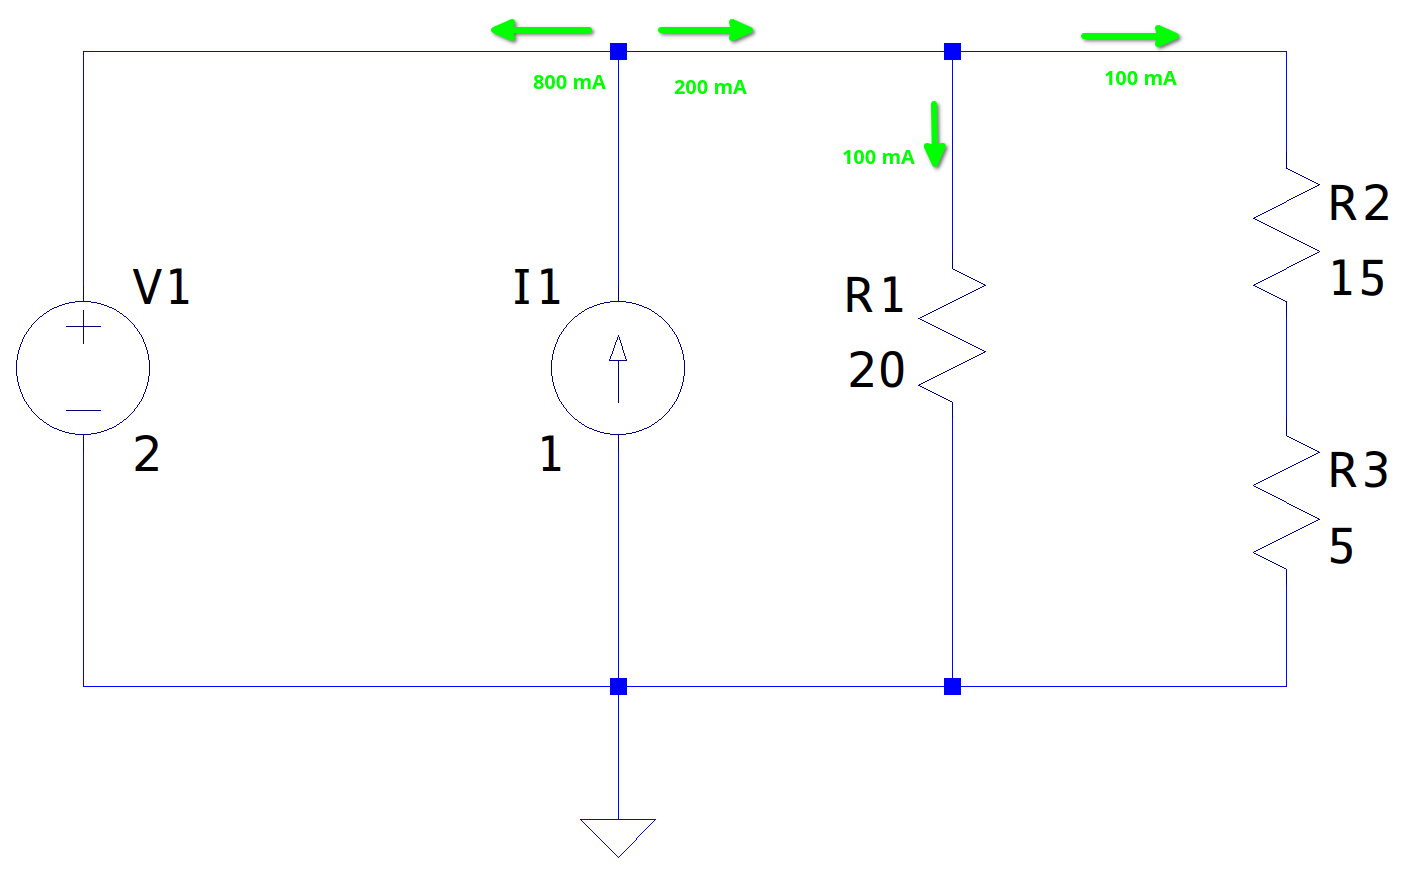
\includegraphics[width=\textwidth]{../pictures/recompose.png} % Pas utiliser width=\textwidth pcq il prend la taille de \section{} comme ref
        \caption{Circuit initial annoté}
    \end{figure}


    \paragraph{}Nous avons donc la première étape de la recomposition de notre circuit avec en vert l'intensité du courant
    (pour le 2ème noeud, j'ai utilisé la loi des noeuds pour déterminer le courant). Nous pouvons calculer la tension aux
    bornes de $R_1$ :

        {\color{info}\begin{align*}
            V_{R_{1}}\;&=\;R \cdot I \\
            V_{R_{1}}\;&=20 \cdot 0.1 \\
            V_{R_{1}}\;&=2
        \end{align*}}
        

        \begin{empheq}[box=\fbox]{equation*}
            \color{red}
            V_{R_{1}}\;=2\;V
        \end{empheq}

    \paragraph{}Ensuite, il faut calculer la tension de $R_2$ et $R_3$. Comme celles-ci sont en série, elles sont traversée
    par la même intensité de courant. Leur tension respective vaut donc :

        {\color{info}\begin{align*}
            V_{R_{2}}\;&=\;R \cdot I \\
            V_{R_{2}}\;&=15 \cdot 0.1 \\
            V_{R_{2}}\;&=1.5
        \end{align*}}
        

        \begin{empheq}[box=\fbox]{equation*}
            \color{red}
            V_{R_{2}}\;=1.5\;V
        \end{empheq}


        {\color{info}\begin{align*}
            V_{R_{3}}\;&=\;R \cdot I \\
            V_{R_{3}}\;&=5 \cdot 0.1 \\
            V_{R_{3}}\;&=0.5
        \end{align*}}
        

        \begin{empheq}[box=\fbox]{equation*}
            \color{red}
            V_{R_{3}}\;=500\;mV
        \end{empheq}
        

\subsection{Calculs des puissances}

        \paragraph{}Il ne nous reste plus qu'a calculé les puissances :

        {\color{info}\begin{align*}
            P_{R_{1}}\;&=\;V \cdot I \\
            P_{R_{1}}\;&=2 \cdot 0.1 \\
            P_{R_{1}}\;&=0.2
        \end{align*}}
        

        \begin{empheq}[box=\fbox]{equation*}
            \color{red}
            P_{R_{1}}\;=200\;mW
        \end{empheq}

        {\color{info}\begin{align*}
            P_{R_{2}}\;&=\;V \cdot I \\
            P_{R_{2}}\;&=1.5 \cdot 0.1 \\
            P_{R_{2}}\;&=0.15
        \end{align*}}
        

        \begin{empheq}[box=\fbox]{equation*}
            \color{red}
            P_{R_{2}}\;=150\;mW
        \end{empheq}


        {\color{info}\begin{align*}
            P_{R_{3}}\;&=\;V \cdot I \\
            P_{R_{3}}\;&=0.5 \cdot 0.1 \\
            P_{R_{3}}\;&=0.05
        \end{align*}}
        

        \begin{empheq}[box=\fbox]{equation*}
            \color{red}
            P_{R_{3}}\;=50\;mW
        \end{empheq}

        {\color{info}\begin{align*}
            P_{V_{1}}\;&=\;V \cdot I \\
            P_{V_{1}}\;&=2 \cdot 0.8 \\
            P_{V_{1}}\;&=1.6
        \end{align*}}
        

        \begin{empheq}[box=\fbox]{equation*}
            \color{red}
            P_{V_{1}}\;=1.6\;W
        \end{empheq}

        {\color{info}\begin{align*}
            P_{I_{1}}\;&=\;V \cdot I \\
            P_{I_{1}}\;&=-2 \cdot 1 \\
            P_{I_{1}}\;&=-2
        \end{align*}}
        

        \begin{empheq}[box=\fbox]{equation*}
            \color{red}
            P_{I_{1}}\;=-2\;W
        \end{empheq}


\section{Tableau récapitulatif}

    \begin{table}[H]
    \centering
    \begin{tabular}{|
    >{\columncolor[HTML]{688FFF}}c |c|c|c|}
    \hline
    / & \cellcolor[HTML]{688FFF}Intensité & \cellcolor[HTML]{688FFF}Tension & \cellcolor[HTML]{688FFF}Puissance \\ \hline
    R1 & 100 mA & 2 V    & 20 mW  \\ \hline
    R2 & 100 mA & 1.5 V  & 150 mW \\ \hline
    R3 & 100 mA & 500 mV & 50 mW  \\ \hline
    V1 & 800 mA & 2 V    & 1.6 W  \\ \hline
    I2 & 1 A    & -2 V   & -2 W   \\ \hline
    \end{tabular}
    \caption{Tableau résumant toutes les données obtenues}
    \label{tab:my-table}
    \end{table}

\section{Conclusion}

    \paragraph{}Pour conclure ce travail, je peux affirmer que les résultats sont accord avec la simulaation du circuit
    faite sur \textit{LTspice}. Ce travail permet de bien mettre en pratique les concepts expliqués au cours magistral.


